\newpage
\section{Auswertung}

Um die aufgenommenen Daten zu analysieren werden die Python~\cite{python} Pakete NumPy~\cite{numpy} und SciPy~\cite{scipy} verwendet,
wobei Matplotlib~\cite{matplotlib} zum Erstellen von Grafiken und zudem Uncertainties~\cite{uncertainties} zur automatisierten
Fehlerfortpflanzung in linearer Ordnung dienen.

Zunächst wird die Koinzidenzschaltung auf ihr zeitliches Auflösungsvermögen geprüft. Weiter muss den Kanälen des Vielkanalanalysators
je eine Zeit zugeordnet werden, bevor mit der eigentlichen Langzeitmessung fortgefahren werden kann.



\subsection{Verzögerungszeit}

Der Verlauf der in Tabelle \ref{tab:delay} gezeigten Messdaten wird in Abbildung \ref{fig:delay} als Trapez mit Null als Asymptote
genähert. Es ergeben sich
\begin{equation*}
	a = \qty{1.7+-0.1}{\per\nano\second}
\end{equation*}
für die Steigung der linken Flanke sowie Knickpunkte
\begin{align*}
	b &= \qty{-11.6+-0.3}{\nano\second} \: , & c &= \qty{-0.1+-0.4}{\nano\second} \: , \\
	d &= \qty{8.1+-0.9}{\nano\second} \: , & e &= \qty{17.3+-0.3}{\nano\second} \: .
\end{align*}

\begin{figure}[H]
	\centering
	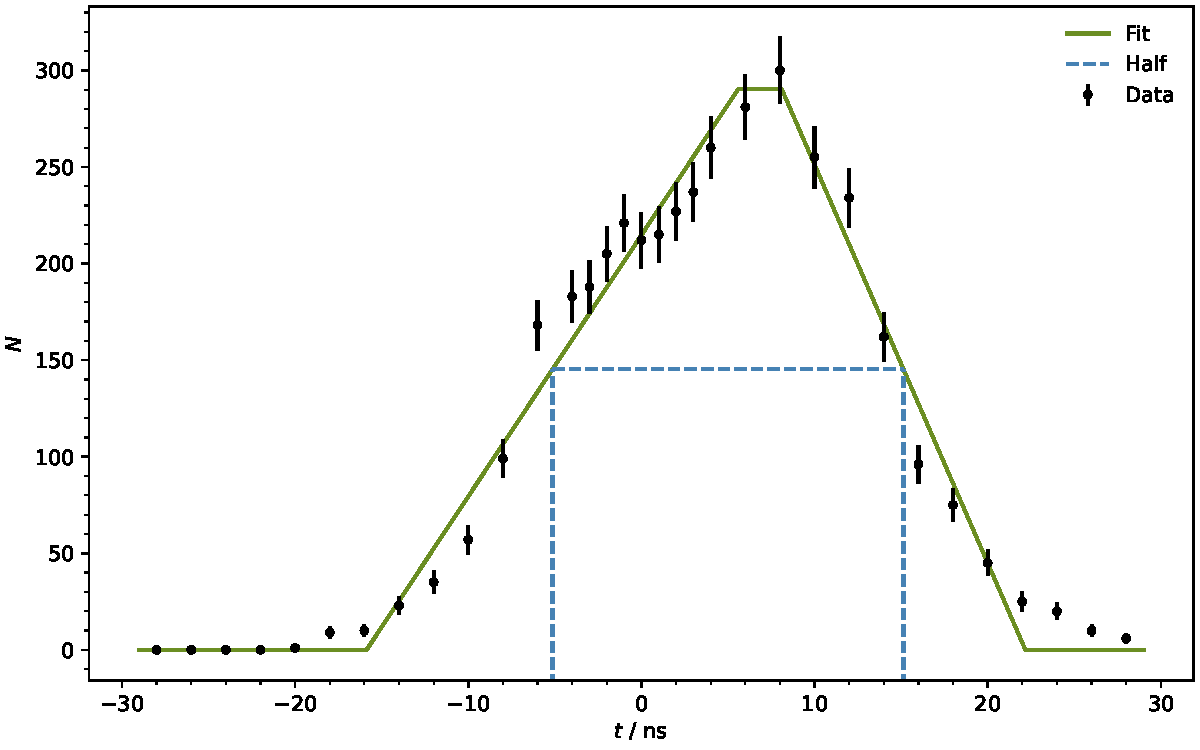
\includegraphics[width=\textwidth]{build/delay.pdf}
	\caption{Gemessene Zählraten gegen die eingestellte Verzögerung.}
	\label{fig:delay}
\end{figure}

Daraus lassen sich einige relevante Größen berechnen. Die maximale Zählrate lautet
\begin{equation*}
	N_\text{Plateau} = \num{20+-1}
\end{equation*}
im Bereich des Plateaus, welches eine Breite
\begin{equation*}
	T_\text{Plateau} = \qty{5.3+-0.5}{\nano\second}
\end{equation*}
aufweist. Die Hälfte dieses Maximums ist bei
\begin{align*}
	t_\text{links} = \qty{-5.9+-0.2}{\nano\second} \: , && t_\text{rechts} = \qty{11.2+-0.2}{\nano\second}
\end{align*}
erreicht. Damit folgt die Halbwertsbreite
\begin{equation*}
	T_\text{Hälfte} = t_\text{rechts} - t_\text{links} = \qty{20.3+-0.8}{\nano\second}
\end{equation*}
und letztendlich eine Auflösungszeit
\begin{equation*}
	T_\text{Auflösung} = T_\text{Hälfte} - T_\text{Plateau} = \qty{11.8+-0.3}{\nano\second} \: .
\end{equation*}



\subsection{Kanalkalibration}

Es wird ein linearer Zusammenhang zwischen Kanalnummer $K$ und der Zeit $t$ angesetzt.

\begin{figure}[H]
	\centering
	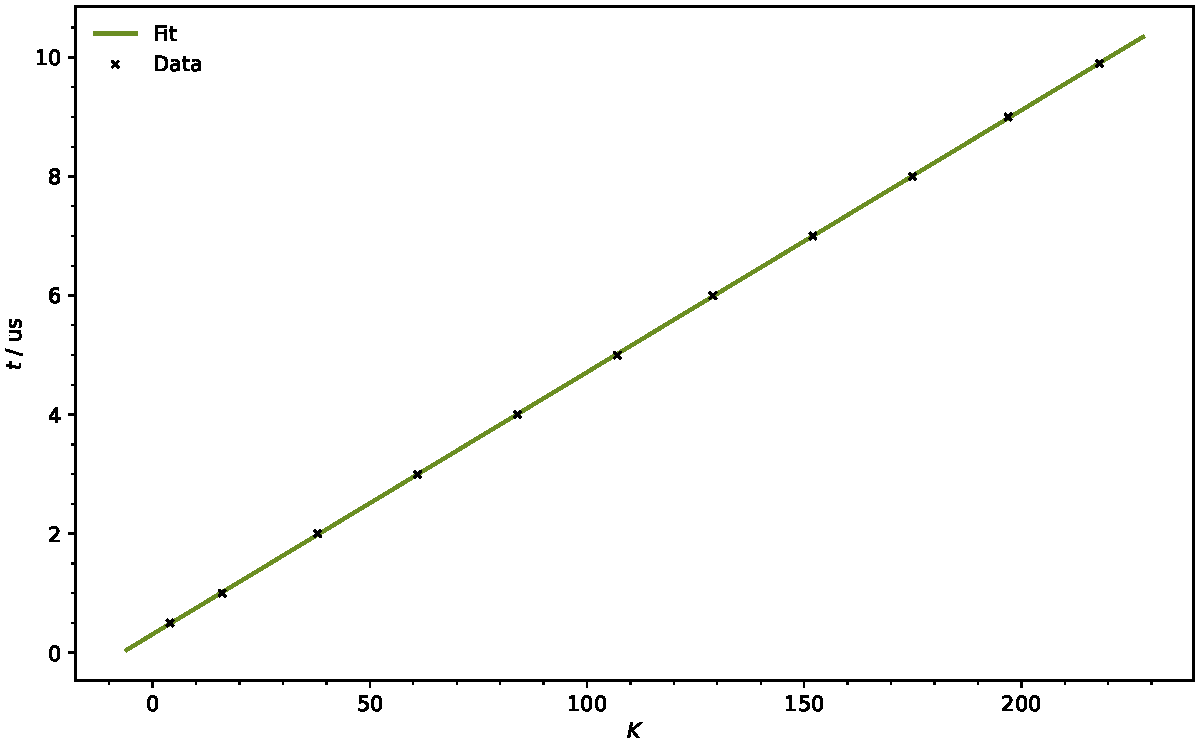
\includegraphics[width=\textwidth]{build/calibration.pdf}
	\caption{Beobachteter Zusammenhang zwischen Kanalnummer und Zeitskala.}
	\label{fig:calibration}
\end{figure}

Aus der entsprechenden Formel für die Ausgleichsrechnung
\begin{equation*}
	t(K) = AK + B
\end{equation*}
bestimmen sich die in Abbildung \ref{fig:calibration} verwendeten Parameter
\begin{align*}
	A = \qty{0.02167+-0.00001}{\micro\second} \: , && B = \qty{0.313+-0.008}{\micro\second}
\end{align*}
zur Umrechnung der Zeitskala aus dem Kanal. Diese Werte ergeben sich, indem an die Daten aus Tabelle \ref{tab:calibration}
angepasst wird.



\subsection{Langzeitmessung}

Für die Messung der Zählrate $N$ gegen die Zeitdifferenz $t$ aus Tabelle \ref{tab:lifetime} lässt sich
\begin{equation*}
	N(t) = m + ne^{-\lambda t}
\end{equation*}
als exponentieller Zusammenhang mit Normierung $n$ ansetzen, der um $m$ als Hintergrund verschoben ist. Aufgrund der
beobachteten Streuung werden ausschließlich die Kanäle mit Indizes $\num{4}$ bis $\num{226}$
verwendet und in Abbildung \ref{fig:lifetime} aufgetragen.

\begin{figure}[H]
	\centering
	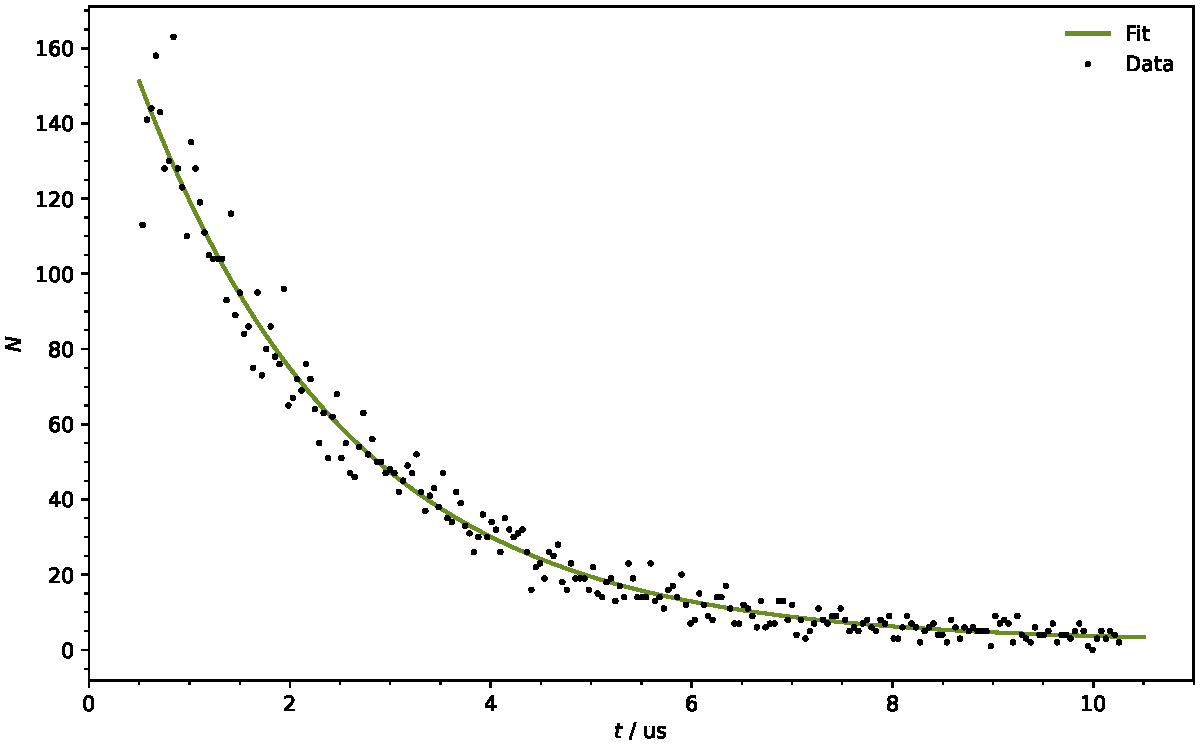
\includegraphics[width=\textwidth]{build/lifetime.pdf}
	\caption{Daten aus der Langzeitmessung mit exponentieller Fitfunktion.}
	\label{fig:lifetime}
\end{figure}

Die Werte der genannten Parameter lauten
\begin{align*}
	m = \num{2.03(0.01)} \: , && n = \num{186.1+-2.7} \: .
\end{align*}
Zusätzlich ergibt sich
\begin{equation*}
	\lambda = \qty{0.44+-0.02}{\per\micro\second}
\end{equation*}
als Zerfallskonstante und schließlich
\begin{equation*}
	\tau = \qty{1.03+-0.03}{\micro\second}
\end{equation*}
für die Lebensdauer kosmischer Myonen, wobei $\qty{2.197}{\micro\second}$ den Literaturwert angibt \cite{Tishchenko_2013}.



\subsection{Hintergrundrate}

Anhand der charakterisierenden Eigenschaften der Messreihe
\begin{align*}
	T_\text{such} &= \qty{10}{\micro\second} \: , & T_\text{mess} &= \qty{158234}{\second} \: , \\
	N_\text{start} &= \num{4509112} \: , & N_\text{stopp} &= \num{17526}
\end{align*}
lässt sich ein Erwartungswert
\begin{equation*}
	\langle N \rangle = N_\text{start} \frac{T_\text{such}}{T_\text{mess}} = \num{0.000285}
\end{equation*}
für die Zählrate innerhalb des Suchzeitintervalls aufstellen. Unter der Annahme einer für Zählexperimente gültigen
Poissonverteilung
\begin{equation*}
	P_k = \pfrac{\langle N \rangle ^k}{k!} e^{-\langle N \rangle}
\end{equation*}
folgt für die Wahrscheinlichkeit, dass genau ein weiteres Myon einfällt,
\begin{equation*}
	P_1 = \qty{0.0191}{\percent} \: .
\end{equation*}
Somit lässt sich die Anzahl zusätzlicher Pulse zu
\begin{equation*}
	O_1 = P_1 N_\text{start} = \num{562}
\end{equation*}
abschätzen, welche sich homogen über $\num{512}$ Kanäle verteilen. Pro Kanal gilt demnach
\begin{equation*}
	M = \num{2.5}
\end{equation*}
als Hintergrundrate, die mit dem Wert $n = \num{2.03(0.01)}$ aus dem vorherigen Vorgehen verglichen werden kann.
